\section{Dynamic Analysis}

Why is the book structured this way?
Chronological vs. non-chronological
How does the structure impact the narrative?

How does the structure evolve throughout the narrative? (dynamic analysis)
Chronological order vs. book order
Attachment: sparsification/densification?
Main character centralities over time

\subsection{Narrative}

\begin{figure*}[ht]
    \centering
    \begin{subfigure}{0.4\textwidth}
        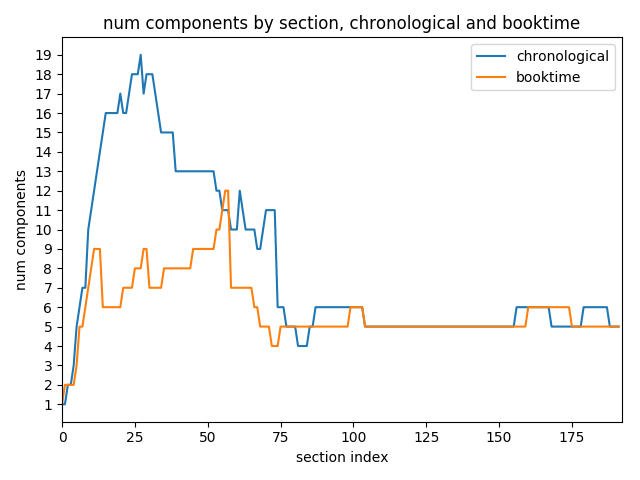
\includegraphics[width=1.\textwidth]{images/dynamics-num-components.png}
        \caption{}
    \end{subfigure}
    \begin{subfigure}{0.4\textwidth}
        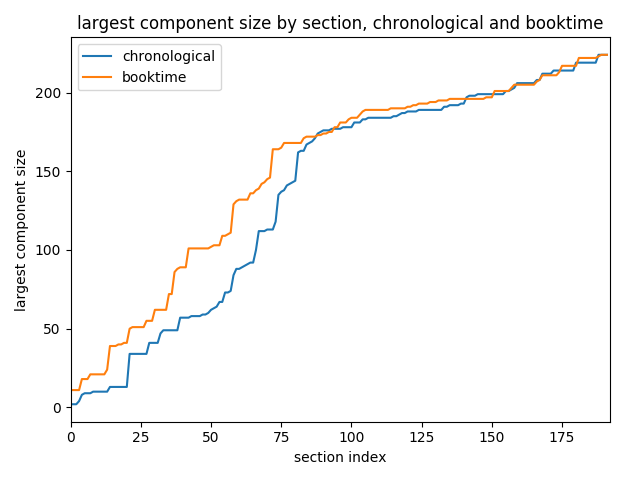
\includegraphics[width=1.\textwidth]{images/dynamics-largest-components.png}
        \caption{}
    \end{subfigure}
    \caption{}
    \label{component-sizes}
\end{figure*}

\subsection{Sparsification vs Densification}
\begin{figure*}[ht]
    \centering
    \begin{subfigure}{0.4\textwidth}
        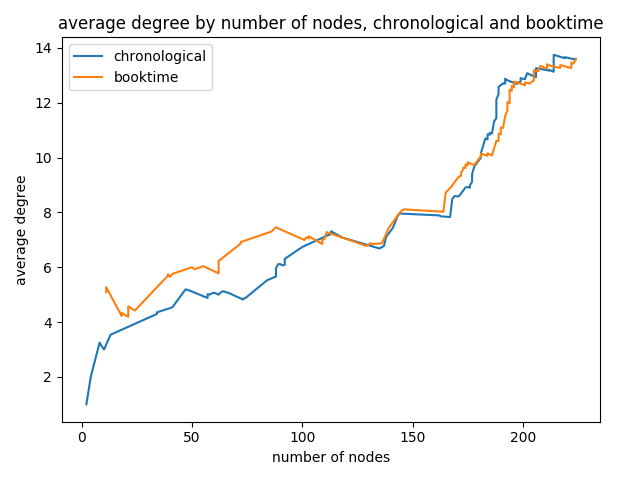
\includegraphics[width=1.\textwidth]{images/n_vs_avg_degree-weighted_False.png}
        \caption{Average unweighted degree in the largest component as a function of nodes}
    \end{subfigure}
    \begin{subfigure}{0.4\textwidth}
        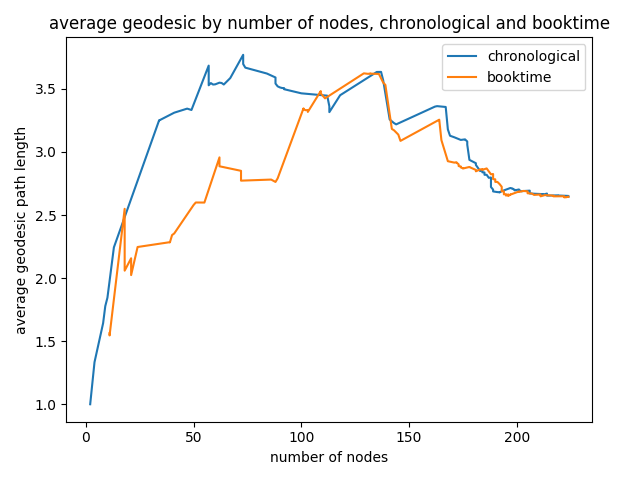
\includegraphics[width=1.\textwidth]{images/n_vs_geodesic-weighted_False.png}
        \caption{Geodesic path length in the largest component as a function of nodes}
    \end{subfigure}
    \caption{Node number's effect on average unweighted degree and geodesic path length in the largest component}
    \label{sparsification-densification}
\end{figure*}

